\subsection{Problem 4: Autoencoder for Utterance Representation}

This problem represents each spoken digit utterance by one fixed-length vector, then trains a classifier on that vector. Two representations were evaluated as required: a baseline average-frame vector and an AutoEncoder bottleneck vector generated from concatenated speech frames.

\subsubsection{Baseline Average-Frame Representation}
For the baseline, each utterance was divided into 15 ms spectrogram frames. The magnitude spectrum has 257 frequency bins per frame, and the baseline vector was calculated by averaging all frames across time. This produces one 257-dimensional vector per utterance. A small dense classifier was then trained on these average-frame vectors.

\subsubsection{AutoEncoder Representation}
For the AutoEncoder approach, all frames of an utterance were concatenated into one vector. The implementation used a fixed analysis length of 100 frames, equivalent to a 25700-dimensional input vector ($100 \times 257$). Shorter utterances were padded with zero frames to match this length. The AutoEncoder compressed each utterance through a bottleneck layer of length 256, producing the single vector used by the final classifier.

The AutoEncoder architecture was:
\[
25700 \rightarrow 1024 \rightarrow 256 \rightarrow 1024 \rightarrow 25700
\]
It was trained for 50 epochs using mean squared reconstruction error. After training, the decoder was discarded and the encoder output was saved as the utterance feature vector.

\begin{figure}[H]
    \centering
    \begin{minipage}{0.48\linewidth}
        \centering
        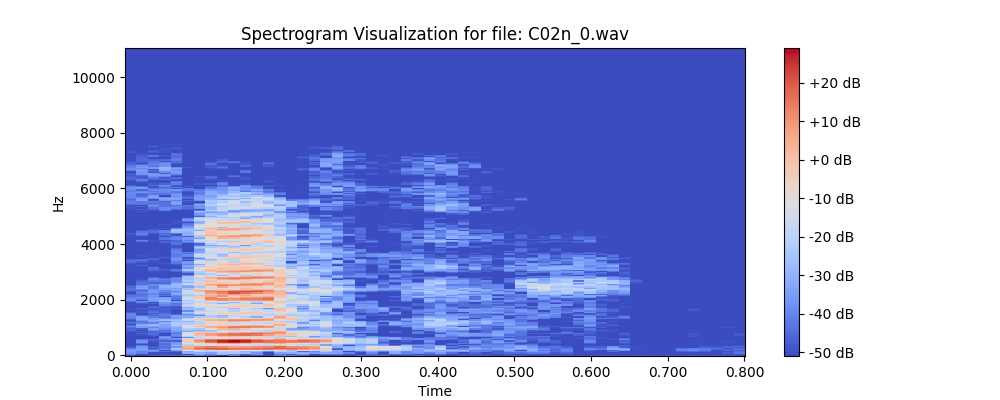
\includegraphics[width=\linewidth]{../Part2_Problem4_AE_Speech/results/Sample_Spectrogram_Visual.png}

        {\small Sample utterance spectrogram}
    \end{minipage}
    \hfill
    \begin{minipage}{0.48\linewidth}
        \centering
        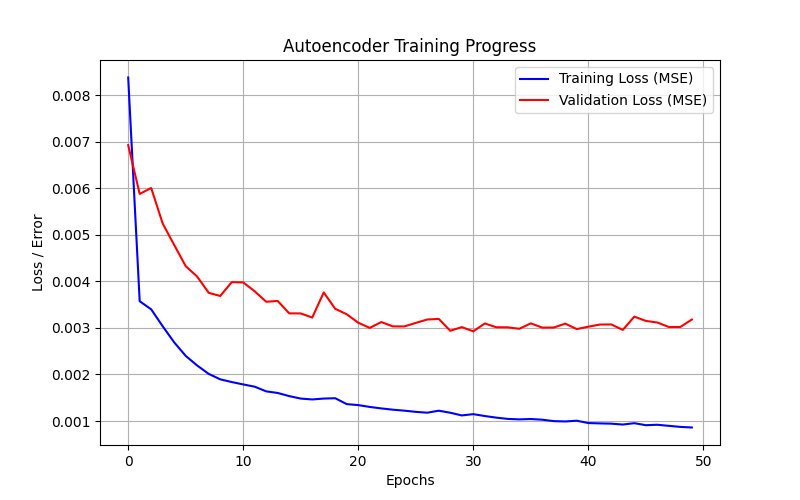
\includegraphics[width=\linewidth]{../Part2_Problem4_AE_Speech/results/Autoencoder_Loss_Curve.png}

        {\small AutoEncoder training and validation loss}
    \end{minipage}
    \caption{Problem 4 input visualization and AutoEncoder reconstruction loss.}
    \label{fig:prob4_ae_inputs}
\end{figure}

\subsubsection{Classifier Results}
The baseline vector and the AutoEncoder bottleneck vector were each passed to dense classifiers. Table~\ref{tab:prob4_results} summarizes the classification performance.

\begin{table}[H]
    \centering
    \caption{Problem 4 utterance-vector classification results}
    \label{tab:prob4_results}
    \resizebox{\linewidth}{!}{
    \begin{tabular}{|l|c|c|c|}
        \hline
        \textbf{Representation / Classifier} & \textbf{Vector Length} & \textbf{Regularization} & \textbf{Test Accuracy} \\
        \hline
        Baseline average frame + dense classifier & 257 & Dropout & 28.3\% \\
        AE bottleneck + 1-hidden-layer MLP & 256 & BatchNorm + Dropout & 78.0\% \\
        AE bottleneck + 3-hidden-layer MLP & 256 & BatchNorm + Dropout & 82.0\% \\
        AE bottleneck + 4-hidden-layer MLP & 256 & BatchNorm + Dropout & 82.0\% \\
        AE bottleneck + 3-hidden-layer MLP, no regularization & 256 & No & 79.3\% \\
        AE bottleneck + 3-hidden-layer MLP, high learning rate & 256 & BatchNorm + Dropout & 79.3\% \\
        \hline
    \end{tabular}
    }
\end{table}

\begin{figure}[H]
    \centering
    \begin{minipage}{0.82\linewidth}
        \centering
        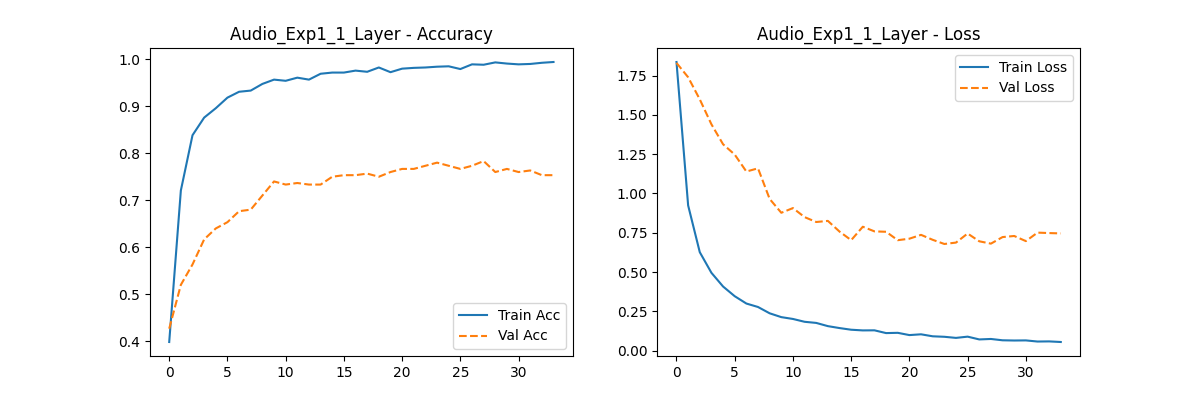
\includegraphics[width=\linewidth]{../Part2_Problem4_AE_Speech/results_after_classification/Audio_Exp1_1_Layer_Curves.png}

        {\small 1 hidden layer}
    \end{minipage}
    \hfill
    \begin{minipage}{0.82\linewidth}
        \centering
        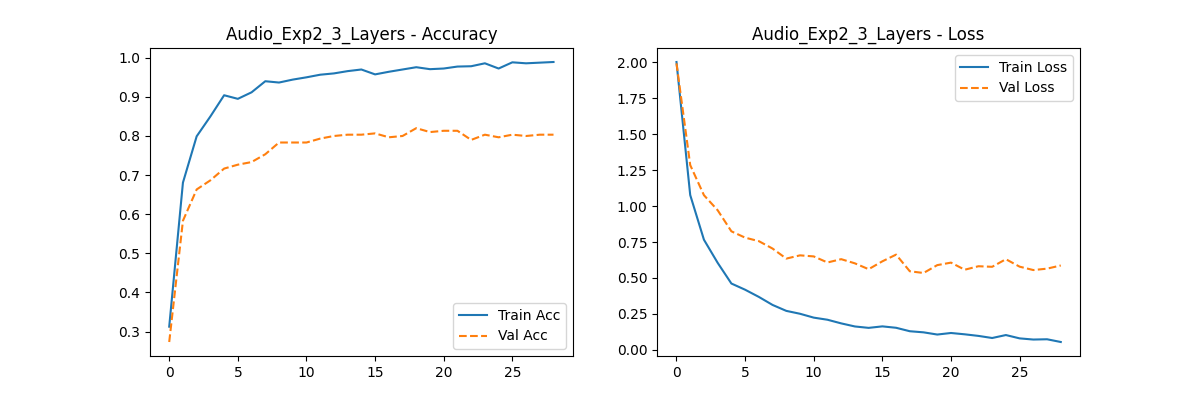
\includegraphics[width=\linewidth]{../Part2_Problem4_AE_Speech/results_after_classification/Audio_Exp2_3_Layers_Curves.png}

        {\small 3 hidden layers}
    \end{minipage}
    \hfill
    \begin{minipage}{0.82\linewidth}
        \centering
        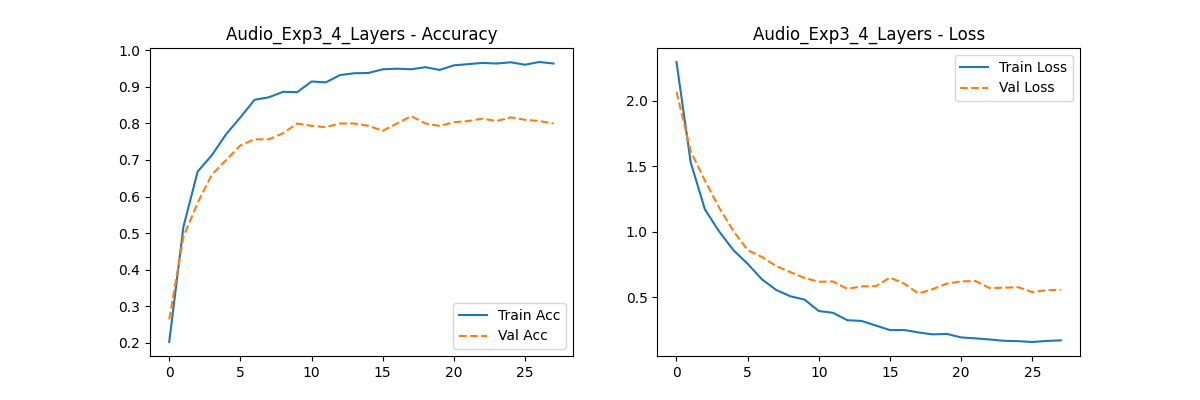
\includegraphics[width=\linewidth]{../Part2_Problem4_AE_Speech/results_after_classification/Audio_Exp3_4_Layers_Curves.png}

        {\small 4 hidden layers}
    \end{minipage}
    \caption{Classifier learning curves using the AutoEncoder bottleneck features.}
    \label{fig:prob4_classifier_curves}
\end{figure}

\subsubsection{Discussion}
The average-frame baseline achieved only $28.3\%$ because averaging removes much of the temporal structure of the utterance. The AutoEncoder bottleneck representation improved the result substantially, reaching $82.0\%$ with both the 3-hidden-layer and 4-hidden-layer classifiers. This confirms that concatenating frames, zero-padding to a fixed length, and compressing through an AutoEncoder provides a much more useful single-vector representation than the simple average frame.
